\section{Functions of Several Variables}

So far all the functions we studied had one
dimensional (scalar) input. Most of the mathematical
models, however, deal with phenomena where the output
depends on several, dependent or independent factors,
hence we need to build and use
functions with multidimensional input; such input is
typically represented as a bundle of scalar variables.

\subsection{Verbal description}

There are several ways in which we can define a
function of several variables. Most times we start with
a \emph{verbal} description, starting from the concrete
situation we want to model and giving specific meanings
to our input and output variables. Here are several examples.

\begin{enumerate}
  \item The apparent temperature, $W$, felt on exposed skin
  depends on several factors, including the actual
  temperature, $T$, the wind speed, $v$, and the humidity.
  The \emph{wind chill temperature} is a mathematical model
  for $W$ under the assumption that the humidity is 0 and
  that the only factors influencing $W$ are $T$ and $v$:
  %
  $$W = W(T,v)\; .$$
  %
  The domain of the function $W$ consists of all reasonable
  pairs $(T,v)$.

  \item The Cobb-Douglas production function models the
  production output, $P$, under the assumption that the
  only factors are the amount of labor, $L$, and the
  amount of capital, $K$:
  %
  $$P=P(L,K) \; .$$

%  \item The magnitude $G$ of the attraction force between
%  two bodies depends on several factors, including the
%  masses $m$ and $M$ of the bodies and the distance $d$
%  between them:
  %
%  $$G=G(m,M,d)$$

  \item A set $(\rho, \phi, \theta)$ of spherical
  coordinates determines the rectangular coordinates
  $(x,y,z)$ of a point. In this case, both the input
  and the output are multidimensional:
  %
  $$(x,y,z) = \textbf{F}(\rho, \theta, \phi)\; ,$$
  %

  \item The wind velocity $\textbf{v}$ at a point $P$
  depends on the position $\textbf{r}$ of $P$,
  %
  $$\textbf{v} = \textbf{V} (\textbf{r})\; .$$
  %
  In this case both the input and the output are
  vectorial quantities.

  \item The electric force on a charge $q$ displaced
  by $\textbf{r}$ from a charge $Q$ depends on the
  two charges, the displacement, and the medium in
  which the charges are placed:
  %
  $$\textbf{E} =
  \textbf{E}(q, Q,\textbf{r})\; .$$
  %
  Note that in this case the output data
  is a vector and the input data is a mix of scalar
  and vectorial quantities.
\end{enumerate}


\subsection{Numerical description}

The verbal description, while essential in understanding
the underlying phenomenon, does not include any quantitative
or visual information. A \emph{numerical} description,
giving output data for a relevant set of input data,
would give additional information and make it easier to
study the mathematical model.

The numerical description is typically given by a table
that contains numerical data collected through experiments
at selected input levels. An example is given by the
Wind Chill Chart provided by NOOA.

%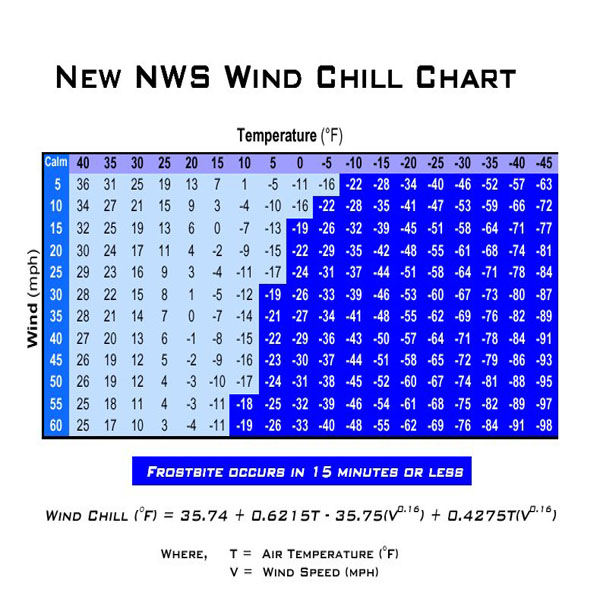
\includegraphics[width=3in]{../images/windchill2.jpg}

Another example is the Income Tax Table. Explain what the
input and output variables are in that case.

\subsection{Analytical description} The numerical
description includes output data only for selected inputs,
so if the actual input values are not among the selected
ones, we will have to approximate by inter/extrapolating
from the given information. To get complete information
we need an \emph{analytical} description, that is, a
procedure to determine the output from any given reasonable
input. This description is typically given through
formulas, and there are several methods of constructing
such formulas.

\begin{enumerate}
  \item For the wind chill, we start with the numerical
  data and simply try to find a function that is defined
  at all intermediary points and that best fits the given
  numerical data. One such example is
  %
  $$W(T,v)= 35.74+0.6215 T - 35.75 v^{0.16} +0.4275 Tv^{0.16}$$
  %
  with $W$ and $T$ in Fahrenheit and $v$ in $mph$.

  \item For the Cobb-Douglas production function, economic
  analysis motivates several properties such a function
  should have, and one model of  a class of functions with
  those properties is
  %
  $$P(K,L) = cL^a K^{1-a}\; ;$$
    %
    here $a$ is a parameter between $0$ and $1$. So, while
    the function $P$ really depends on three variables $a$,
    $L$, and $K$, we treat the variables differently: we
    consider $a$ to be a parameter of the model, and once
    we decide on the value of $a$, we treat it as a constant.

    \item The transition formulas from spherical to
    rectangular coordinates are given by geometric reasoning.

    \item An important class of functions of several variables
    is the class of
    polynomial functions. Polynomials
    of degree one are
    %
    \begin{align*}
    f(x,y) = & ax+by+c \\
      g(x,y,z) = & ax+by+cz+d  \; ,
    \end{align*}
    %
    and polynomials of degree two are
    \begin{align*}
      f(x,y) = & \; a_{11}x^2+a_{12}xy+a_{22}y^2+ a_1 x + a_2 y + a_0 \\
      g(x,y,z) = & \; a_{11} x^2 + a_{22}y^2 + a_{33}z^2 + a_{12}xy + a_{13}xz+a_{23}yz + \\
      & + a_1 x + a_2 y + a_3 z + a_0
    \end{align*}
    %
    where the $a_{ij}$'s are real numbers.

    \item The formula for electric force is given by
    laws of physics: the magnitude of the force is directly
    proportional to the charges $q$, $Q$, and inversely
    proportional to the square of the distance between them.
    The force acts along the line joining the two points,
    attracts $q$ to $Q$ if the charges have different sign
    and rejects $q$ from $Q$ if the charges have the same
    sign. The mathematical translation is
    %
    $$\textbf{E}(q, Q, \textbf{r}, \epsilon) =
    \frac{\epsilon q Q}{|\textbf{r}|^3} \textbf{r}\; ,$$
    %
    where $\epsilon$ is a proportionality constant,
    depending on the medium the charges are placed in.
\end{enumerate}

\section{Graphical descriptions}

\subsection{Functions of two variables}
While an analytical description technically provides
complete information, it does it in a not so easy to
interpret form. For example, if the output is a scalar,
where does the function attain its extreme values? And
how do the values change for nearby points? Are they
decreasing, increasing? How fast? We will learn how to
decode  that information, but even then, it would be much
more clarifying if we had a picture showing all that
information at once.

\vspace{1cm}
\begin{center}
  Figure: Graph of a scalar function
\end{center}
\vspace{1cm}

For a function of one variable, $y=f(x)$, the graph of
$f$ is a set of points in $\RR^2$, more precisely,
the set of points $(x,y)$ such that $y=f(x)$.
For example, if $f(x) = x^2$, then  $(3,9)$ is on the
graph, because $9=3^2$, but $(2,5)$ is not, because
$5 \neq 2^2$.

We can extend this graphical representation for
functions with two dimensional input and one dimensional
output. The \emph{graph} of the function
$f\colon D \to \RR$, where $D$ is a region in $\RR^2$,
is the set of points $P(x,y,z)$ in $\RR^3$ whose
coordinates satisfy the condition $z=f(x,y)$.

For example, the graph of $f(x,y) = 2x-y+3$ is the set
%
$$\{ (x,y,z) \, | \, z= 2x-y+3\} \Longrightarrow
\text{ plane } 2x-y-z+3=0 \; .$$


\subsection{Slices and level curves}
A slightly more complicated example is
$g(x,y) =x^2+2y^2$. What does the
graph of $g$ look like?

By definition, the graph $\Gamma$ of $g$ is the set of points
$P(x,y,z)$ in $\RR^3$ such that $z=x^2+2y^2$. This is
no longer linear, so the set is not a plane. But what
does it look like?

A method that provides significant insight is to use
sections. The graph of $g$ lives in $\RR^3$ and we
use an imaginary CT scan to cut it, understand the
sections, and re-assemble the sections
in order to get the graph.

What does it means to cut the graph by vertical planes
parallel to the $Oyz-$plane? Such a plane has equation
$x=a$, for some constant $a$. The intersection of such
a plane with the graph $\Gamma$ is given by points of
coordinates $(a, y, z=a^2+2y^2)$, and those points form
a parabola in the plane $x=a$, with vertex at
$(a,0,a^2)$. The vertex rises as $a$ gets away from 0.
Intersecting the graph of $g$ with the plane $x=a$ means
essentially that we treat $x$ as a constant, and we study
the partial function $y\to z=g(a,y) = a^2+2y^2$.

Similarly, if we cut by planes $y=a$ we get partial
functions $x\to x^2+2a^2$, whose graphs are also
parabolas. Each such a parabola is now situated in the
vertical plane $y=a$. Hence vertical sections are
parabolas, with vertices rising as
we move farther away from the coordinate planes.

To get horizontal sections we have to
keep constant not an input variable, but the output
variable, $z$. Intersecting the graph of $g$ with
the plane $z=a$ we get a curve of equations $x^2+2y^2=a$,
$z=a$. For $a<0$ the intersection is empty, for $a=0$ it
consists of a single point, $(x,y,z) = (0,0,0)$, and for
$a>0$, the intersection is an ellipse in the plane $z=a$.

The \emph{level curve} corresponding to $z=a$ is the curve
$g(x,y)=a$ in the domain of $g$, with a label $a$ to
indicate the level of the output corresponding to
that level curve. Note that the level curve is not the
intersection of the graph of $g$ with the plane $z=a$;
instead, it is the projection of that intersection onto
the plane $Oxy$, where the domain of $g$ resides.

You should be familiarized with level curves if
you have ever seen a topographic map or if you
opened the newspaper at the weather section. What are the
functions in those cases?


\subsection{Level sets}
The examples considered in the previous sections were all
examples of functions with scalar output and a two
dimensional input. Their graphs lived in
$\RR^3 = \RR^{2+1}$, with the 2 coming from the dimension
of the input and the 1 from the dimension of the output.
If we wanted to extend that graphic construction to
functions depending on three scalar variables,
we'd need $3+1=4$ dimensions for the graphs, and that
is momentarily impossible. The rescue comes from the
second graphical representation, using level sets,
because the level sets (with appropriate labeling of
the level) can be represented in a space with dimension
equal to the dimension of the input space.


For example, let $f(x,y,z) = ax+by-z$. The graph is the
quadruple $(x,y,z,w)$ in $\RR^4$ such that
$w = ax+by-z$, and we can't yet represent that
graphically. But the level set $f(x,y,z) = d$ is the
surface $ax+by-z = d$ in $\RR^3$, and that surface is a
plane. Level sets corresponding to equidistant values
$d_1$, $d_2$, and $d_3$ of the output are parallel
planes of equations
%
\begin{align*}
  \mathcal{P}_1 = f^{-1}(d_1) & \colon \; ax+by-z = d_1\\
  %
  \mathcal{P}_2 = f^{-1}(d_2) & \colon \; ax+by-z = d_2\\
  %
  \mathcal{P}_3 = f^{-1}(d_3) & \colon \; ax+by-z = d_3
\end{align*}
%
and these planes are also equidistant.

The following remark will play a very important role in
understanding surfaces in space.

\begin{rmk}{\rm The level set $f(x,y,z)=0$ for the
function
%
$$f(x,y,z) = ax+by-z+d$$
%
is the same as the graph
of the function $g(x,y) = ax+by+c$.
}\end{rmk}

We will see that while graph surfaces can always be
represented as level surfaces, the converse is not true:
level surfaces can't always be represented as graph
surfaces. However, we'll show that under some reasonable
assumptions, level surfaces can \emph{locally} be
described as graph surfaces. An illuminating example is
that of a sphere (centered at the origin): it is the
level surface of $f(x,y,z) = x^2+y^2+z^2$, but it can't
be globally represented as a graph surface. Try and see
what goes wrong!



\subsection{Vector fields} We conclude this section
with an introduction to \emph{vector fields}.
These are examples of functions with multidimensional
input and output. The
input is identified with a point in space,
and the output is represented as a vector with
the tail at that point. Examples of vector fields include:

\begin{itemize}
  \item Velocity of fluid/air at given point;
  \item Electric force per unit of charge;
  \item Gravitational field;
  %\item Fundamental directions $\textbf{e}_\rho$, $\textbf{e}_\phi$, $\textbf{e}_\theta$, $\textbf{e}_r$
\end{itemize}

In rectangular coordinates a vector field $\textbf{F}$ can
be decomposed along the fundamental directions,
%
$$\textbf{F}(x,y,z) = F_1(x,y,z) \textbf{i} + F_2(x,y,z) \textbf{j} + F_3(x,y,z) \textbf{k} \; .$$
%
If we deal with regions in the plane, then we have similar
concepts and definitions for 2-dimensional vector fields.
For example the vector field $\textbf{e}_r$ is given by
%
$$\textbf{e}_r = \cos\theta\, \textbf{i} +
\sin\theta \,\textbf{j} = \frac{x}{r} \, \textbf{i} +
\frac{y}{r} \, \textbf{j} = \frac{x}{\sqrt{x^2+y^2}} \,
\textbf{i} + \frac{y}{\sqrt{x^2+y^2}} \, \textbf{j}$$
%
and is defined on $\mathbb{R}^2 \setminus \{ (0,0)\}$.
Similarly the vector field $\textbf{e}_{\theta}$ is
%
$$\textbf{e}_\theta = -\sin\theta\, \textbf{i} +
\cos\theta \,\textbf{j} = -\frac{y}{r} \, \textbf{i} +
\frac{x}{r} \, \textbf{j} = -\frac{y}{\sqrt{x^2+y^2}} \,
\textbf{i} + \frac{x}{\sqrt{x^2+y^2}} \, \textbf{j} \; .$$
%
 \begin{center}
\begin{tabular}{cc}
  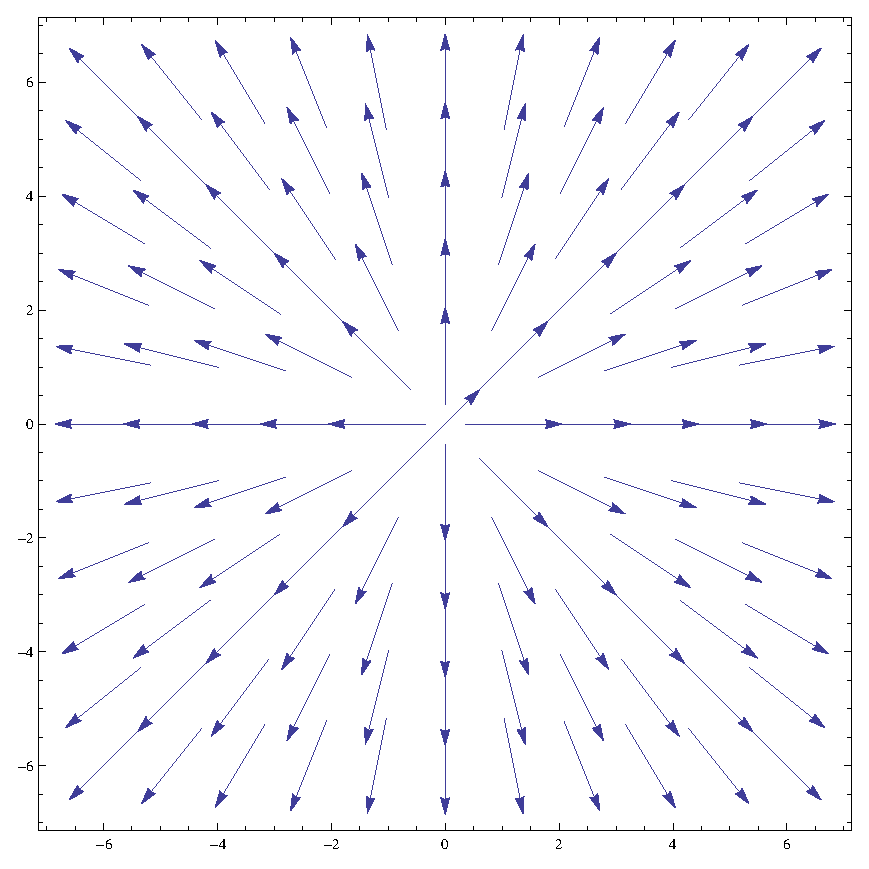
\includegraphics[height=5cm]{../images/radial_field.eps}
  &
  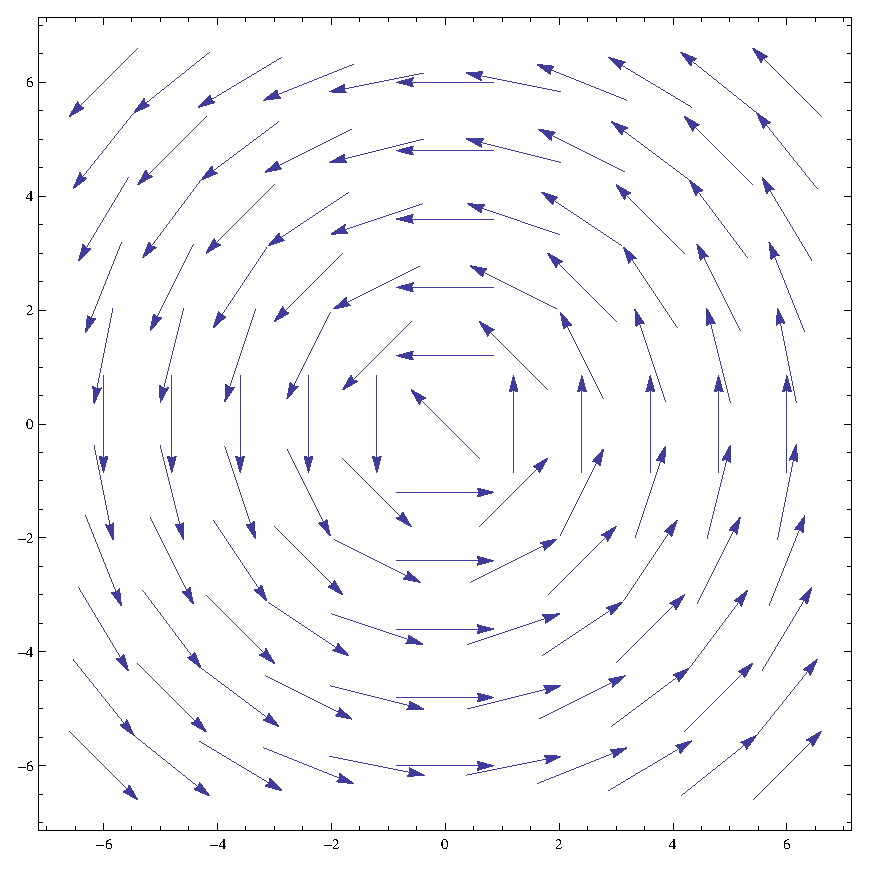
\includegraphics[height=5cm]{../images/rotational_field.eps}
  \\
  Radial field $\textbf{e}_r$ & Rotational field
  $\textbf{e}_\theta$
\end{tabular}
\end{center}

The graphical representations of these vector fields makes
it quite clear what would happen to an object forced to move
so that the velocity at each point is given by the value of
the field.

Similar to decomposition in rectangular coordinates
we can decompose a vector field along fundamental vectors
corresponding to other coordinate systems. Things are a bit
trickier, since the fundamental vectors change from
point to point.

In particular, a planar vector field can be written in terms of
$\textbf{e}_r$ and $\textbf{e}_\theta$:
%
$$\textbf{X}(r,\theta) = X_1(r,\theta) \textbf{e}_r\, +
X_2(r,\theta) \textbf{e}_\theta\; .$$
%
For example, if $X(P) = \textbf{i}$, then
%
$$X(r,\theta) = \cos\theta \,\textbf{e}_r\,
-\sin\theta \, \textbf{e}_\theta\; .$$


%%%%%%%%%%%%%%%%%%


%%%%%%%%%%%%%%%%%%%%%%%%

\section{Surfaces}

\subsection{Quadric Surfaces}

Level sets for second degree polynomial functions

$$f(x,y,z) = Ax^2+By^2+Cz^2+Dxy+Exz+Fyz+Gx+Hy+Iz+J$$

\begin{itemize}
  \item At least one of $A$, $B$, $C$, $D$, $E$, or $F$ is non-zero;
  \item Some coefficients may be zero.
\end{itemize}

Level set $f(x,y,z)=k$ is called a \emph{quadric surface}. It suffices to consider $k=0$.

Through rigid motions (translations and rotations) it can be reduced to one of the following canonical forms (for different values of $A$, $B$, and $C$):
%
$$
  Ax^2+By^2+Cz^2+D = 0 \quad \text{ or } \quad
  Ax^2+By^2+Iz=0
$$
%
with not all of $A$, $B$, and $C$ equal to zero and $I$ not zero.

\begin{equation*}
Ax^2+By^2+Cz^2+D = 0
\end{equation*}

\begin{table}
\begin{tabular}{|c|c|c|c|c|c|c|c|c|}
  \hline
  % after \\: \hline or \cline{col1-col2} \cline{col3-col4} ...
  A & B & C & D & $x=x_0$ & $y=y_0$ & $z=z_0$ & Example & Name
  \\
  \hline
  $>0$ & $>0$ & $>0$ & $>0$ & empty & empty & empty & $x^2+2y^2+3z^2+4=0$ & empty \\
  \hline
  $>0$ & $>0$ & $>0$ & $=0$ &  &  &  &  &  \\
  \hline
  $>0$ & $>0$ & $>0$ & $<0$ & ellipse & ellipse & ellipse & $x^2+2y^2+3z^2-4=0$ & Ellipsoid \\
  \hline
  $>0$ & $>0$ & $=0$ & $>0$ &  &  &  &  &  \\
  \hline
  $>0$ & $>0$ & $=0$ & $=0$ &  &  &  &  &  \\
  \hline
  $>0$ & $>0$ & $=0$ & $<0$ &  &  &  &  &  \\
  \hline
  $>0$ & $>0$ & $<0$ & $>0$ &  &  &  &  &  \\
  \hline
  $>0$ & $>0$ & $<0$ & $=0$ &  &  &  &  &  \\
  \hline
  $>0$ & $>0$ & $<0$ & $<0$ &  &  &  &  &  \\
  \hline
  $>0$ & $=0$ & $=0$ & $>0$ &  &  &  &  &  \\
  \hline
  $>0$ & $=0$ & $=0$ & $=0$ &  &  &  &  &  \\
  \hline
  $>0$ & $=0$ & $=0$ & $<0$ &  &  &  &  &  \\
  \hline
\end{tabular}
\caption{Quadrics with central symmetry}
\end{table}

Fill in the rest of the table.

\bigskip


\begin{equation*}
Ax^2+By^2+Iz=0
\end{equation*}

\begin{table}
\begin{tabular}{|c|c|c|c|c|c|c|}
  \hline
  % after \\: \hline or \cline{col1-col2} \cline{col3-col4} ...
  A & B  & $x=x_0$ & $y=y_0$ & $z=z_0$ & Example & Name
  \\
  \hline
  $>0$ & $>0$   & parabola & parabola & ellipse, point, or empty & $x^2+2y^2+3z=0$ & Elliptic paraboloid \\
  \hline
  $>0$ & $=0$ & &  &  &  &   \\
  \hline
  $>0$ & $<0$ &  &  &  &  &   \\
  \hline
\end{tabular}
  \caption{Quadrics without central symmetry}
\end{table}
\bigskip

Fill in the rest of the table.


\subsection{Implicit functions}

A surface $S$ can be given in two different ways:

\begin{itemize}
  \item Implicit form, as a \emph{level surface}:
  %
  $$F(x,y,z) = k$$
  %
  \item  Explicit form, as a \emph{graph surface}:
  %
  $$z=f(x,y) \Longrightarrow \left\{ \begin{array}{ll}
    x = & u \\
    y = & v \\
    z = & f(u,v)
  \end{array} \right.$$
\end{itemize}

A graph surface $z=f(x,y)$ can always be represented as a level surface:
%
$$z=f(x,y) \Longleftrightarrow F(x,y,z) =0 \quad \text{ for } \quad F(x,y,z) = z-f(x,y)\; .$$

\underline{Question}: Can a given level surface be represented as a graph surface?

The answer to the question above is two-fold:

\begin{itemize}
  \item Bad news: In general, \emph{globally}, NO.

  \noindent Think $x^2+y^2+z^2= 1$.

  One can't solve for $z$ globally; there is the $\pm\sqrt{1-x^2-y^2}$ issue;
  \item Good news: In a lot of situations, \emph{locally}, YES.

  \noindent Around $P(0,0,1)$, the surface is the graph surface of $z = \sqrt{1-x^2-y^2}$.
\end{itemize}

Consider a function $F(x,y,z)$, let $P(x_0,y_0,z_0)$ be a point in the domain of $F$, and let $k=F(x_0,y_0,z_0)$. The level surface through $P$, of equation $F(x,y,z) = k$ is a graph surface around $P$ if there is a function $z=f(x,y)$ such that:
%
\begin{itemize}
  \item $f$ is defined on an open disk $D$ around $(x_0,y_0)$;
  \item $f(x_0,y_0) = z_0$;
  \item $F(x,y,f(x,y)) = 0$ for all $(x,y)$ in the disk $D$.
\end{itemize}

If that is the case, we say that the equation $F(x,y,z) = k$ \emph{implicitly} defines $z=f(x,y)$ satisfying the condition $f(x_0,y_0) = z_0$.

Examples:

The equation $x^2+y^2+z^2 = 1$ implicitly defines $z=\sqrt{1-x^2-y^2}$ as the unique function $z=f(x,y)$ such that
%
\begin{itemize}
  \item $x^2+ y^2+(f(x,y))^2 = 1$ for all $(x,y)$ in a disk around $(0,0)$;
  \item $f(0,0) = 1$.
\end{itemize}

The equation $x^2+y^2+z^2 = 1$ implicitly defines $z=-\sqrt{1-x^2-y^2}$ as the unique function $z=f(x,y)$ such that
%
\begin{itemize}
  \item $x^2+ y^2+(f(x,y))^2 = 1$ for all $(x,y)$ in a disk around $(0,0)$;
  \item $f(0,0) = -1$.
\end{itemize}

\subsection{Parametrizations}
So far we have focused our attention on functions with
a scalar output. However, we have already seen examples of
functions with vectorial output, and one such example is
involved in the vectorial parametric equation of a plane.

If $\mathcal{P}$ is the plane through
$P_0(\textbf{r}_0)$ and parallel to directions
$\textbf{u}$ and $\textbf{v}$, then the points
of $\mathcal{P}$ have position vectors $\textbf{r}$
satisfying
%
$$\textbf{r} = \textbf{r}_0 + s \textbf{u} +
t \textbf{v}\; ,$$
%
so the function $\bm{f} \colon \RR^2 \to \RR^3$,
$\bm{f}(s,t) = \textbf{r}_0 +
s \textbf{u} + t \textbf{v}$ globally identifies
$\RR^2$ with the plane $\mathcal{P}$.
Each point $P$ of $\mathcal{P}$ corresponds
uniquely to a pair of coordinates $(s,t)$.

Another important example of a function with a
two dimensional input and a three dimensional output is
the following.

\begin{exmp}{\rm Let $f \colon (0,2\pi)
\times (0,\pi) \to \RR^3$ be given by
%
$$f(t,s) = (R\sin{s}\cos{t}, R\sin{s}\sin{t},
R\cos{s}) \; .$$
%
Then the image of $f$ is a subset of the
sphere of radius $R$ centered at the origin.
Which points of the sphere are not covered
by the image of $f$?
}\end{exmp}


% % % % % % % % % % % % % % % % % % % % %